\documentclass[landscape,final,a0paper,fontscale=0.277]{baposter}

\usepackage{calc}
\usepackage{graphicx}
\usepackage{amsmath}
\usepackage{amssymb}
\usepackage{relsize}
\usepackage{multirow}
\usepackage{rotating}
\usepackage{bm}
\usepackage{url}

\usepackage{graphicx}
\usepackage{multicol}
\usepackage{siunitx}

%\usepackage{times}
%\usepackage{helvet}
%\usepackage{bookman}
\usepackage{palatino}
\newcommand\Tstrut{\rule{0pt}{2.6ex}}         % = `top' strut

\newcommand{\captionfont}{\footnotesize}

\graphicspath{{images/}{../images/}}
\usepackage{tikz}
\usetikzlibrary{shapes.misc}
\usetikzlibrary{shapes,arrows,decorations.markings,shadows,positioning}

\newcommand{\SET}[1]  {\ensuremath{\mathcal{#1}}}
\newcommand{\MAT}[1]  {\ensuremath{\boldsymbol{#1}}}
\newcommand{\VEC}[1]  {\ensuremath{\boldsymbol{#1}}}
\newcommand{\Video}{\SET{V}}
\newcommand{\video}{\VEC{f}}
\newcommand{\track}{x}
\newcommand{\Track}{\SET T}
\newcommand{\LMs}{\SET L}
\newcommand{\lm}{l}
\newcommand{\PosE}{\SET P}
\newcommand{\posE}{\VEC p}
\newcommand{\negE}{\VEC n}
\newcommand{\NegE}{\SET N}
\newcommand{\Occluded}{\SET O}
\newcommand{\occluded}{o}

%%%%%%%%%%%%%%%%%%%%%%%%%%%%%%%%%%%%%%%%%%%%%%%%%%%%%%%%%%%%%%%%%%%%%%%%%%%%%%%%
%%%% Some math symbols used in the text
%%%%%%%%%%%%%%%%%%%%%%%%%%%%%%%%%%%%%%%%%%%%%%%%%%%%%%%%%%%%%%%%%%%%%%%%%%%%%%%%

%%%%%%%%%%%%%%%%%%%%%%%%%%%%%%%%%%%%%%%%%%%%%%%%%%%%%%%%%%%%%%%%%%%%%%%%%%%%%%%%
% Multicol Settings
%%%%%%%%%%%%%%%%%%%%%%%%%%%%%%%%%%%%%%%%%%%%%%%%%%%%%%%%%%%%%%%%%%%%%%%%%%%%%%%%
\setlength{\columnsep}{1.5em}
\setlength{\columnseprule}{0mm}

%%%%%%%%%%%%%%%%%%%%%%%%%%%%%%%%%%%%%%%%%%%%%%%%%%%%%%%%%%%%%%%%%%%%%%%%%%%%%%%%
% Save space in lists. Use this after the opening of the list
%%%%%%%%%%%%%%%%%%%%%%%%%%%%%%%%%%%%%%%%%%%%%%%%%%%%%%%%%%%%%%%%%%%%%%%%%%%%%%%%
\newcommand{\compresslist}{%
	\setlength{\itemsep}{1pt}%
	\setlength{\parskip}{0pt}%
	\setlength{\parsep}{0pt}%
}

%%%%%%%%%%%%%%%%%%%%%%%%%%%%%%%%%%%%%%%%%%%%%%%%%%%%%%%%%%%%%%%%%%%%%%%%%%%%%%
%%% Begin of Document
%%%%%%%%%%%%%%%%%%%%%%%%%%%%%%%%%%%%%%%%%%%%%%%%%%%%%%%%%%%%%%%%%%%%%%%%%%%%%%

\begin{document}


%%%%%%%%%%%%%%%%%%%%%%%%%%%%%%%%%%%%%%%%%%%%%%%%%%%%%%%%%%%%%%%%%%%%%%%%%%%%%%
%%% Here starts the poster
%%%---------------------------------------------------------------------------
%%% Format it to your taste with the options
%%%%%%%%%%%%%%%%%%%%%%%%%%%%%%%%%%%%%%%%%%%%%%%%%%%%%%%%%%%%%%%%%%%%%%%%%%%%%%
\definecolor{lightblue}{rgb}{0.145,0.6666,1}

\definecolor{silver}{cmyk}{0,0,0,0.3}
\definecolor{black}{cmyk}{0,0,0.0,1.0}
\definecolor{darkYellow}{cmyk}{0,0,1.0,0.5}
\definecolor{darkSilver}{cmyk}{0,0,0,0.1}

\definecolor{KTHBlue}{cmyk}{.71,.37,0.07,0}
\definecolor{KTHsilver}{cmyk}{0,0,0,0.35}
\definecolor{KTHbeige}{cmyk}{0,0.03,0.19,0.04}

% Argonne Logo Colors
\definecolor{ArgoneLogoBlue}{RGB}{4,146,210}
\definecolor{ArgoneLogoRed}{RGB}{228,32,41}
\definecolor{ArgoneLogoGreen}{RGB}{120,202,42}
\definecolor{PMSCoolGray}{RGB}{112,109,110}

% \definecolor{KTHBlue}{RGB}{25,84,166}
\begin{poster}{
  % Poster Options
	% Show grid to help with alignment
	grid=false,
	% Column spacing
	colspacing=1em,
	% Color style
	bgColorOne=white,
	bgColorTwo=white,
	borderColor=lightblue,
	headerColorOne=black,
	headerColorTwo=lightblue,
	headerFontColor=white,
	boxColorOne=white,
	boxColorTwo=lightblue,
	% Format of textbox
	textborder=roundedleft,
	% Format of text header
	eyecatcher=true,
	headerborder=closed,
	headerheight=0.13\textheight,
	%  textfont=\sc, An example of changing the text font
	headershape=roundedright,
	headershade=shadelr,
	headerfont=\Large\bf\textsc, %Sans Serif
	textfont={\setlength{\parindent}{1.5em}},
	boxshade=plain,
	%  background=shade-tb,
	background=plain,
	linewidth=2pt
}
% Eye Catcher
{
\includegraphics[height=6em]{./logos/Argonne_cmyk_black}} 
% Title
{\bf\textsc{Photoinjector Optimization for the Argonne Wakefield Accelerator Facility}}%\vspace{0.1em}}
% Authors
{Nicole Neveu and Linda Spentzouris, IIT \\
Jeffrey Larson and John Power, ANL}
% University logo
{% The makebox allows the title to flow into the logo, this is a hack because of the L shaped logo.

\includegraphics[height=4.0em]{./logos/IIT_logo}
}


%%%%%%%%%%%%%%%%%%%%%%%%%%%%%%%%%%%%%%%%%%%%%%%%%%%%%%%%%%%%%%%%%%%%%%%%%%%%%%
%%% Now define the boxes that make up the poster
%%%---------------------------------------------------------------------------
%%% Each box has a name and can be placed absolutely or relatively.
%%% The only inconvenience is that you can only specify a relative position 
%%% towards an already declared box. So if you have a box attached to the 
%%% bottom, one to the top and a third one which should be in between, you 
%%% have to specify the top and bottom boxes before you specify the middle 
%%% box.
%%%%%%%%%%%%%%%%%%%%%%%%%%%%%%%%%%%%%%%%%%%%%%%%%%%%%%%%%%%%%%%%%%%%%%%%%%%%%%
  %
  % A coloured circle useful as a bullet with an adjustably strong filling
  \newcommand{\colouredcircle}[1]{%
    \tikz{\useasboundingbox (-0.2em,-0.32em) rectangle(0.2em,0.32em); \draw[draw=black,fill=baposterBGone!80!black!#1!white,line width=0.03em] (0,0) circle(0.18em);}}

%%%%%%%%%%%%%%%%%%%%%%%%%%%%%%%%%%%%%%%%%%%%%%%%%%%%%%%%%%%%%%%%%%%%%%%%%%%%%%
\headerbox{Abstract}{name=problem,column=0,row=0}{
%%%%%%%%%%%%%%%%%%%%%%%%%%%%%%%%%%%%%%%%%%%%%%%%%%%%%%%%%%%%%%%%%%%%%%%%%%%%%%
A strength of model-based, derivative-free, trust-region optimization algorithms 
is their efficient use of function evaluations. We use one such 
algorithm, BOBYQA, to optimize the beam dynamics in two cases of interest at 
the Argonne Wakefield Accelerator (AWA) facility. First we model the complete 
AWA rf photoinjector at 40 nC with. The optimization algorithm is used 
in a Pareto study that compares the trade-off 
between emittance and bunch length for the AWA 70 MeV photoinjector. Second, 
we compare BOBYQA to a genetic algorithm (GA), which is a popular optimization 
technique in the field.  
}

%%%%%%%%%%%%%%%%%%%%%%%%%%%%%%%%%%%%%%%%%%%%%%%%%%%%%%%%%%%%%%%%%%%%%%%%%%%%%%
\headerbox{Simulation Model and Optimization Variables}{name=sims,column=1,row=0,span=2}{
%%%%%%%%%%%%%%%%%%%%%%%%%%%%%%%%%%%%%%%%%%%%%%%%%%%%%%%%%%%%%%%%%%%%%%%%%%%%%%
\def \gunleft {-1.0}
\def \gunright {0.3}
%This should say "left", but I'm lazy and didn't change it
\def \loneright {1.0}
\def \ltworight {3.5}
\def \lthreeright {5.0}
\def \lfourright {7.0}
\def \lfiveright {8.5}
\def \lsixright {10}
%\centering
\begin{center}
	\begin{tikzpicture}[scale=0.75]
	%Gun drawings
	%{\textbf{$S_1, S_2$}  %{\textbf{$S_1, S_2$} % {\textbf{$S_3$}}
	\draw[fill=orange, very thick, rounded corners =0.1cm] (\gunleft,0.5)rectangle (\gunright,1.5) node[pos=.5, white] {\textbf{Gun}} ;
	
	%S1
	\node[] at (-1.3,2.9) {$S_1$};
	\draw[ultra thick, fill=black!60!green] (-1.4,-0.5)rectangle  (-1.0,0.5) node[pos=.5, white] {} ;
	\draw[black, ultra thick] (-1.4,-0.5) -- (-1.0,0.5);
	\draw[black, ultra thick] (-1.4,0.5) -- (-1.0,-0.5);
	\draw[ultra thick, fill=black!60!green] (-1.4,1.5)rectangle  (-1.0,2.5) node[pos=.5, white] {} ;
	\draw[black, ultra thick] (-1.4,1.5) -- (-1.0,2.5);
	\draw[black, ultra thick] (-1.4,2.5) -- (-1.0,1.5);
	%S2
	\node[] at (-0.8,2.9) {$S_2$};
	\draw[ultra thick, fill=black!60!green] (-1.0,-0.5)rectangle  (-0.6,0.5) node[pos=.5, white] {} ;
	\draw[black, ultra thick] (-1.0,-0.5) -- (-0.6,0.5);
	\draw[black, ultra thick] (-1.0,0.5) -- (-0.6,-0.5);
	\draw[ultra thick, fill=black!60!green] (-1.0,1.5)rectangle  (-0.6,2.5) node[pos=.5, white] {} ;
	\draw[black, ultra thick] (-1.0,1.5) -- (-0.6,2.5);
	\draw[black, ultra thick] (-1.0,2.5) -- (-0.6,1.5);
	
	%S3
	\node[] at (0.2,2.9) {$S_3$};
	\draw[ultra thick, fill=black!60!green] (-0.1,-0.5) rectangle  (0.3,0.5) node[pos=.5, white] {};
	\draw[black, ultra thick] (-0.1,-0.5) -- (0.3,0.5);
	\draw[black, ultra thick] (-0.1,0.5) -- (0.3,-0.5);
	\draw[ultra thick, fill=black!60!green] (-0.1,1.5) rectangle  (0.3,2.5) node[pos=.5, white] {};
	\draw[black, ultra thick] (-0.1,1.5) -- (0.3,2.5);
	\draw[black, ultra thick] (-0.1,2.5) -- (0.3,1.5);
	%Linac drawings 
	\draw[fill=blue, ultra thick, rounded corners =0.1cm] (\loneright,0)rectangle  ({\loneright+0.84},2) node[pos=.5, white] {$L_1$} ;
	\draw[fill=blue, ultra thick, rounded corners =0.1cm] (\ltworight,0)rectangle  ({\ltworight+0.84},2) node[pos=.5, white] {$L_2$};
	\draw[fill=blue, ultra thick, rounded corners =0.1cm] (\lthreeright,0)rectangle ({\lthreeright+0.84},2) node[pos=.5, white] {$L_3$};
	\draw[fill=blue, ultra thick, rounded corners =0.1cm] (\lfourright,0)rectangle ({\lfourright+0.84},2) node[pos=.5, white] {$L_4$};
	\draw[fill=blue, ultra thick, rounded corners =0.1cm] (\lfiveright,0)rectangle ({\lfiveright+0.84},2) node[pos=.5, white] {$L_5$};
	\draw[fill=blue, ultra thick, rounded corners =0.1cm] (\lsixright,0)rectangle ({\lsixright+0.84},2) node[pos=.5, white] {$L_6$};
	\draw[very thick] (\gunleft,-1.5) -- (14,-1.5);
	%\path [draw=black, fill=black] (1,-2.5) circle (2pt); %black circle
	%\path [draw=black, fill=white, thick] (2,-2.5) circle (2pt); %white circle
	\draw[latex-latex] (\gunleft,-1.5) -- (14,-1.5) ;
	\foreach \x in  {0.3, 1.0, 3.5, 5.0, 7.0, 8.5, 10, 12.5} %tick marks
	\draw[shift={(\x,-1.5)},color=black] (0pt,3pt) -- (0pt,-3pt);
	\foreach \x in {0.3, 1.0, 3.5, 5.0, 7.0, 8.5, 10, 12.5}
	\draw[shift={(\x,-1.7)},color=black] (0pt,0pt) node[below]
	{$\x$};
	
	\node[draw, fill=yellow, star, star points=5, star point ratio=0.6, minimum size=0.6cm]
	at (12.5,1.0) {$z_1$};
	\end{tikzpicture}
\end{center}

\noindent
\begin{minipage}{0.425\textwidth}
	$S_1$--$S_3$ refer to gun solenoids, and~$L_1--L_6$ to accelerating cavities.
	The location of optimization is $z_1=\SI{12.51}{m}$.
	The 10 parameters, $v=[S_3, \phi_g, R, T, \phi_L]$, were varied during linac simulations. 
	Note:~$\phi_L~=~[\phi_{L_1},\ldots,\phi_{L_6}]$. 
\end{minipage} \hfill
\begin{minipage}{0.55\textwidth}
	\centering
	\begin{tabular}{ l *{3}{c}}
		%\toprule
		\textbf{Variable} & \textbf{Range} & \textbf{Unit} \\
		\hline %\midrule
		Solenoid Strength & $ 0 \le S_3 \le 440$  & amps \Tstrut \\
		Phase of Gun & $-60 \le \phi_g \le 60$  & degrees \\
		Laser Radius  & $0.1 \le R \le 30$  & mm \\
		Laser FWHM  & $2 \le T \le $10  & ps \\
		Cavity Phase & $-20 \le \phi_L \le 20$  & degrees
		%\bottomrule    
	\end{tabular}
\end{minipage}

}

%%%%%%%%%%%%%%%%%%%%%%%%%%%%%%%%%%%%%%%%%%%%%%%%%%%%%%%%%%%%%%%%%%%%%%%%%%%%%%
\headerbox{Optimization Algorithm}{name=diagram,column=0,below=problem}{
%%%%%%%%%%%%%%%%%%%%%%%%%%%%%%%%%%%%%%%%%%%%%%%%%%%%%%%%%%%%%%%%%%%%%%%%%%%%%%
Given a candidate optimal set of parameters $v^k$, BOBYQA
constructs a quadratic model using function values of points near $v^k$. This
model is minimized in a neighborhood of $v^k$ in order to produce a point $\hat{v}$. 
If $\hat{v}$ has a smaller objective function value than $v^k$, the estimate of the optimum is
updated to $\hat{v}$, and a new model is constructed. If $\hat{v}$ is not a
sufficient improvement over $v^k$, the model around $v^k$ is improved. 
}

%%%%%%%%%%%%%%%%%%%%%%%%%%%%%%%%%%%%%%%%%%%%%%%%%%%%%%%%%%%%%%%%%%%%%%%%%%%%%%
\headerbox{Source Code}{name=code,column=0,below=diagram}{%, bottomaligned=conclusion}{
%%%%%%%%%%%%%%%%%%%%%%%%%%%%%%%%%%%%%%%%%%%%%%%%%%%%%%%%%%%%%%%%%%%%%%%%%%%%%%
Beam dynamics were simulated with the open source particle-in-cell code OPAL-t. 
The optimization was performed using the open source package NLopt 
in combination with Python code written at ANL.
All the files needed to replicate the results in this poster are available at:
\noindent
\begin{center}
	\url{www.mcs.anl.gov/~jlarson/AWA}
\end{center}
%\vspace{0.01cm}
}
%%%%%%%%%%%%%%%%%%%%%%%%%%%%%%%%%%%%%%%%%%%%%%%%%%%%%%%%%%%%%%%%%%%%%%%%%%%%%%
\headerbox{Acknowledgements}{name=doe,column=0,below=code, above=bottom}{
%%%%%%%%%%%%%%%%%%%%%%%%%%%%%%%%%%%%%%%%%%%%%%%%%%%%%%%%%%%%%%%%%%%%%%%%%%%%%%
We gratefully acknowledge the computing resources
provided on Blues, a HPC cluster operated by the LCRC at ANL.
This work is supported by the U.S. DOE, Office of Science, under
contract number DE-AC02-06CH11357 and grant number DE-SC0015479.

}



%%%%%%%%%%%%%%%%%%%%%%%%%%%%%%%%%%%%%%%%%%%%%%%%%%%%%%%%%%%%%%%%%%%%%%%%%%%%%%
\headerbox{Genetic Algorithms(GA)}{name=multiple,column=3,row=0,span=1}{
%%%%%%%%%%%%%%%%%%%%%%%%%%%%%%%%%%%%%%%%%%%%%%%%%%%%%%%%%%%%%%%%%%%%%%%%%%%%%%
Pareto fronts for both the larger and tighter domains. 
\centering
\begin{tabular}{ l *{3}{c}}
	%\toprule
	\textbf{Variable} & \textbf{Range} & \textbf{Unit} \\
	\hline 
	Solenoid Strength & $ 0 \le S_3 \le 440$  & amps \Tstrut \\
	Phase of Gun & $-60 \le \phi_g \le 60$  & degrees \\
	Laser Radius  & $0.1 \le R \le 30$  & mm \\
	Laser FWHM  & $2 \le T \le $10  & ps \\
	Cavity Phase & $-20 \le \phi_L \le 20$  & degrees
	%\bottomrule    
\end{tabular}
\begin{center}
	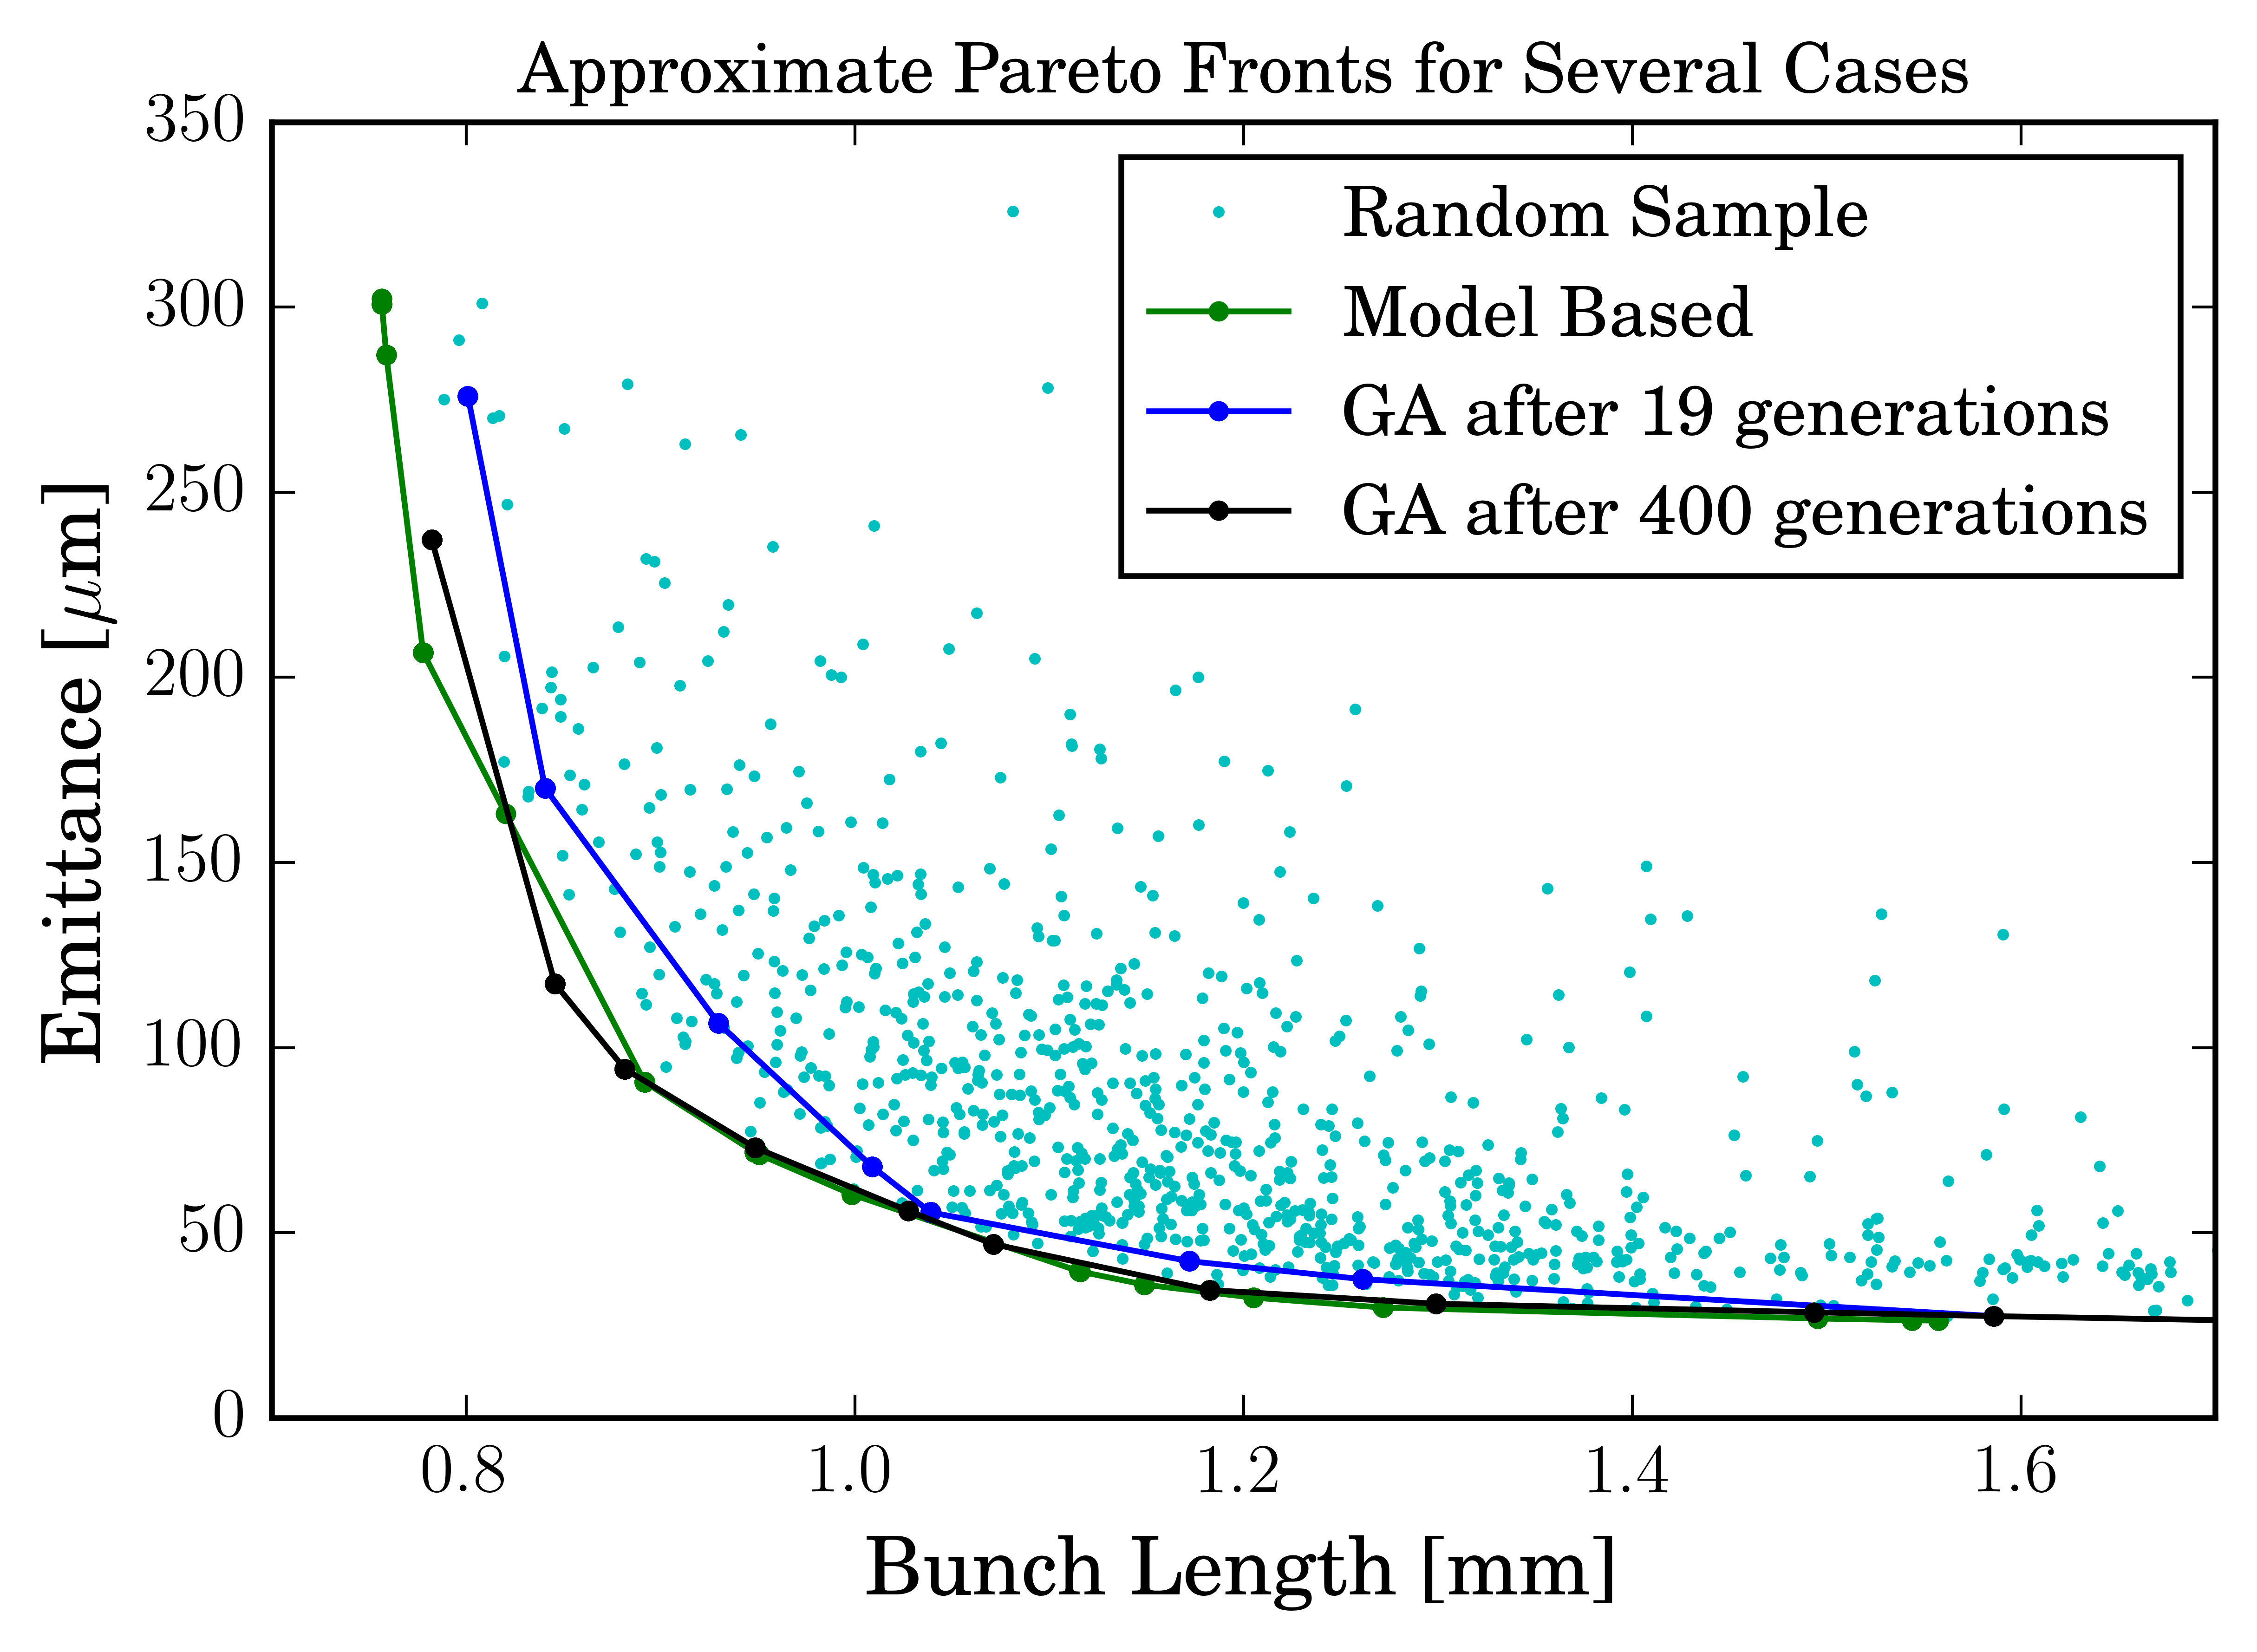
\includegraphics[width=0.9\textwidth]{./images/pareto_emittance_vs_zrms}
\end{center}

}

%%%%%%%%%%%%%%%%%%%%%%%%%%%%%%%%%%%%%%%%%%%%%%%%%%%%%%%%%%%%%%%%%%%%%%%%%%%%%%
\headerbox{Linac Optimization}{name=conditions,below=sims,column=1,row=0,span=2}{
%%%%%%%%%%%%%%%%%%%%%%%%%%%%%%%%%%%%%%%%%%%%%%%%%%%%%%%%%%%%%%%%%%%%%%%%%%%%%%
\noindent
\begin{minipage}{0.5\textwidth}
	Out of a 1,000 point sample, 132 simulations completed without error.
	From the 132-point set, the min and max values of $\epsilon_{x}(v,w)$ and $\sigma_{z}(v,w)$ were found.
	All set values were then shifted and scaled:
	\begin{align*}
	\bar{\epsilon}_x (v,z_1) = \frac{ \epsilon_x (v,z_1) - \epsilon_{\min} } { \epsilon_{\max} - \epsilon_{\min} }
	\end{align*}
	This scaling is done to remove the difference in the units between
	$\epsilon_x(v,w)$ and $\sigma_z(v,w)$. An approximate Pareto front 
	was constructed by solving eleven optimization problems, 
	$f(v,w)$, that ranged from pure emittance optimization $(w~=~1)$ to pure bunch length optimization $(w~=~0)$.
	For each weight $w$, BOBYQA was started from the sample point with the smallest value of $f(v,w)$.
	\begin{gather*}
	w\in\left\{ 0, 0.1, \ldots, 1 \right\}\\
	f(v,w) = w \,\bar{\epsilon}_x(v,z_1) + (1-w)\, \bar{\sigma}_z(v,z_1)
	\end{gather*}
	In total, 2,492 simulation evaluations produced the approximate Pareto front.
	Most evaluations took ~7-10 minutes, using 16 cores and 100,000 particles.
\end{minipage}
\begin{minipage}[t]{0.5\textwidth}
	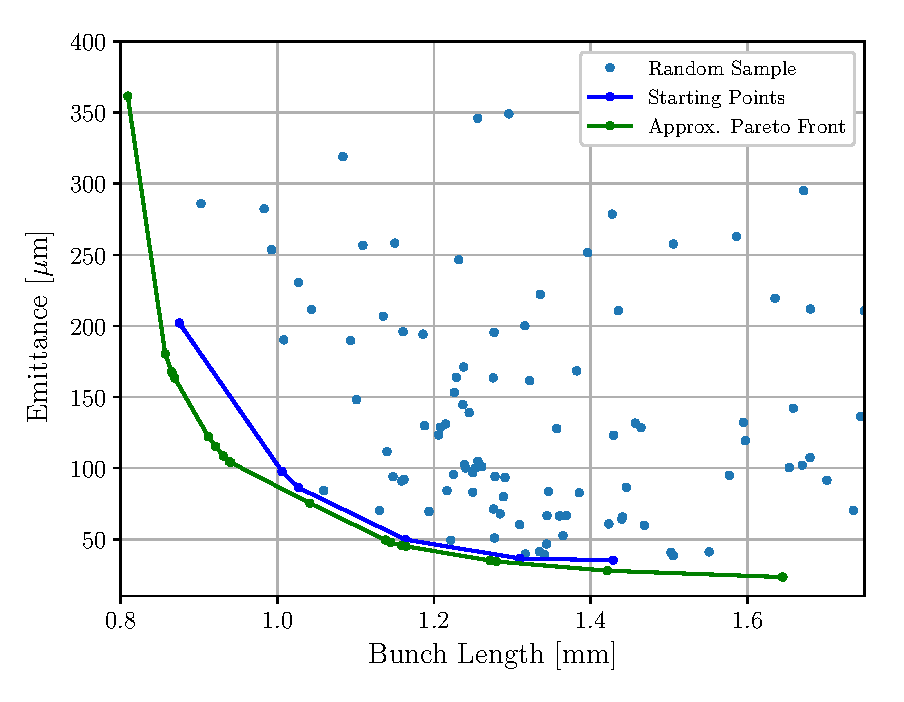
\includegraphics[width=0.9\textwidth]{./images/THPAB155f1}
	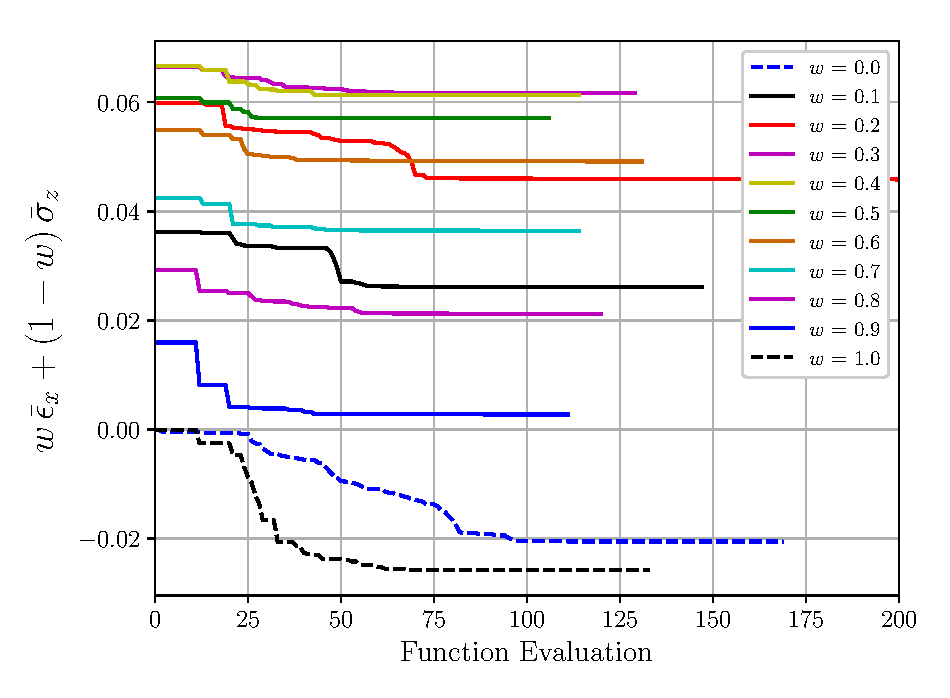
\includegraphics[width=0.9\textwidth]{./images/THPAB155f2}
\end{minipage}




\iffalse
\begin{minipage}[t]{0.5\textwidth}

\end{minipage}\hspace{0.2cm}
\begin{minipage}[t]{0.5\textwidth}


\end{minipage}
\fi
}




%%%%%%%%%%%%%%%%%%%%%%%%%%%%%%%%%%%%%%%%%%%%%%%%%%%%%%%%%%%%%%%%%%%%%%%%%%%%%%
\headerbox{Conclusion}{name=conclusion,column=3,below=multiple, span=1}{%
%%%%%%%%%%%%%%%%%%%%%%%%%%%%%%%%%%%%%%%%%%%%%%%%%%%%%%%%%%%%%%%%%%%%%%%%%%%%%%
We used BOBYQA to perform a multiobjective analysis for the linac at \SI{40}{nC}.
We then compared those results to a GA. This analysis will be used to 
decide future operating parameters at the AWA during high-charge experiments.
Future work will include a refinement of results using 3D field maps for all
cavities, and experimental measurements to verify the results.
%\begin{center}
%\includegraphics[width=0.9\linewidth]{DOE_logo_color_cmyk}
%\end{center}
}

\end{poster}%
%
\end{document}
